\documentclass[11pt,a4paper]{article}
\usepackage[top=1.8cm,bottom=1.8cm,left=1.9cm,right=1.9cm]{geometry}
\usepackage{booktabs}
\usepackage{graphicx}
\usepackage{amsmath}
\usepackage{hyperref}
\usepackage{listings}
\usepackage{xcolor}
\usepackage{caption}
\usepackage{float}
\usepackage{parskip}

\lstset{
  language=Python,
  basicstyle=\ttfamily\scriptsize,
  keywordstyle=\color{blue},
  commentstyle=\color{gray},
  breaklines=true,
  frame=single,
  numbers=left,
  numberstyle=\tiny,
  aboveskip=4pt,
  belowskip=4pt,
}

\title{\textbf{Replication Report: Deep Reinforcement Learning for\\
Automated Stock Trading --- An Ensemble Strategy}\\[0.5em]
\large Financial Analytics and Machine Learning}
\author{Student ID: zczq358}
\date{May 2026}

\begin{document}
\maketitle
\thispagestyle{empty}

%──────────────────────────────────────────────────────────────────
\section{Description of the Paper}
%──────────────────────────────────────────────────────────────────

Yang et al.\ (2020) address the problem of designing a profitable and
risk-aware automated stock trading strategy in a complex, dynamic market.
Rather than relying on return prediction, they cast portfolio management as a
\textbf{Markov Decision Process (MDP)} and use deep reinforcement learning to
learn a trading policy that directly maximises cumulative portfolio value.

\textbf{MDP formulation.}
The state at time $t$ is $s_t = [b_t, \mathbf{p}_t, \mathbf{h}_t, \mathbf{M}_t,
\mathbf{R}_t, \mathbf{C}_t, \mathbf{X}_t]$: available balance, adjusted close
prices, share holdings, and four technical indicators (MACD, RSI, CCI, ADX)
for each of the 30 DJIA stocks, yielding a 181-dimensional state vector.
The action is a continuous vector $\mathbf{a}\in[-k,k]^{30}$ representing
shares to buy (positive) or sell (negative) for each stock.
The reward is the change in total portfolio value minus a 0.1\% transaction
cost. A financial turbulence index (Mahalanobis distance of current returns
from historical mean) is used to trigger full liquidation during extreme market
events.

\textbf{Algorithms.}
Three actor-critic algorithms are trained concurrently: \textit{Proximal Policy
Optimisation} (PPO), \textit{Advantage Actor-Critic} (A2C), and
\textit{Deep Deterministic Policy Gradient} (DDPG).

\textbf{Ensemble strategy.}
Every quarter, a growing training window is used to retrain all three agents.
Each agent is then validated on a 3-month rolling window, and the agent with
the highest Sharpe ratio is deployed for trading over the next quarter. This
adaptive selection allows the ensemble to switch between agents depending on
prevailing market conditions.

\textbf{Original results.}
Over the out-of-sample period 2016--2020, the ensemble achieves a Sharpe ratio
of 1.30, cumulative return of 70.4\%, and maximum drawdown of $-9.7\%$,
outperforming all three individual agents as well as the DJIA index (Sharpe
0.47) and a min-variance portfolio (Sharpe 0.45).

%──────────────────────────────────────────────────────────────────
\section{Python Implementation}
%──────────────────────────────────────────────────────────────────

\textbf{Data.}
Daily OHLCV data for 29 DJIA constituent stocks (UTX was delisted) from
2009-01-01 to 2020-05-08 were downloaded via \texttt{yfinance}.
MACD, RSI, CCI, and ADX were computed using the \texttt{ta} library with the
same window parameters as the paper. The turbulence index uses a rolling
252-day Mahalanobis distance.

\textbf{Environment.}
A custom \texttt{gymnasium} environment implements the 175-dimensional state
space, continuous action space $[-1,1]^{29}$ (scaled by $H_{\max}=100$
shares), 0.1\% transaction cost, and turbulence-triggered liquidation
(threshold = 140). The reward is the normalised daily change in portfolio value.

\begin{lstlisting}[caption={Environment step: sells first then buys; turbulence guard liquidates all holdings.}]
def step(self, action):
    acts = (action * self.hmax).astype(int)
    if self.turb[self.day] > self.turb_thr:   # risk-aversion
        acts = -self.shares.astype(int)
    for i in np.where(acts < 0)[0]:           # sell
        sell_sh = min(-acts[i], int(self.shares[i]))
        self.balance += sell_sh * prices[i] * (1 - self.tc)
    for i in np.where(acts > 0)[0]:           # buy
        buy_sh = min(acts[i], int(self.balance / (prices[i]*(1+self.tc))))
        self.balance -= buy_sh * prices[i] * (1 + self.tc)
    reward = (portfolio_value_new - portfolio_value_prev) / self.init_bal
\end{lstlisting}

\textbf{Training.}
PPO and A2C were trained for 150,000 timesteps each; DDPG for 80,000 steps,
all using a two-hidden-layer MLP (256$\times$256) and learning rate $10^{-4}$.
Agents were trained \emph{once} on the in-sample period (2009--2015).

\textit{Key simplification:} The paper retrains all agents every quarter using
a growing window. Due to computational constraints, we train once and implement
only the quarterly \emph{selection} step, re-using the fixed models.

\textbf{Ensemble selection.}
At the start of each quarter $q$, the agent with the highest Sharpe ratio over
quarter $q-1$ is selected for deployment in quarter $q$, identical to the
paper's Step 2--3 logic (see Appendix, Figure~\ref{fig:selection}).

\textbf{Min-variance baseline.}
The minimum-variance portfolio is constructed analytically using the full
in-sample return covariance matrix $\hat{\Sigma}$ estimated from daily returns
over 2009--2015 (approximately 1,700 observations). Optimal weights are given
by $w^* = \hat{\Sigma}^{-1}\mathbf{1} \,/\, (\mathbf{1}^\top\hat{\Sigma}^{-1}\mathbf{1})$,
clipped to be non-negative (long-only constraint) and then renormalised.
Weights are fixed at inception and \emph{not} rebalanced during the trading
period; shares are purchased at 2016-01-04 prices and held throughout.
This buy-and-hold design means the portfolio drifts away from its optimal
weights over time, which underestimates the performance a quarterly-rebalanced
min-variance strategy would achieve.

%──────────────────────────────────────────────────────────────────
\section{Results}
%──────────────────────────────────────────────────────────────────

Figure~\ref{fig:cumret} shows cumulative returns from 2016-01-04 to
2020-05-08. Table~\ref{tab:perf} compares our replication with the original
paper. The DJIA index serves as the primary benchmark, downloaded directly via
the \texttt{\^{}DJI} ticker to ensure accuracy.

\begin{figure}[H]
  \centering
  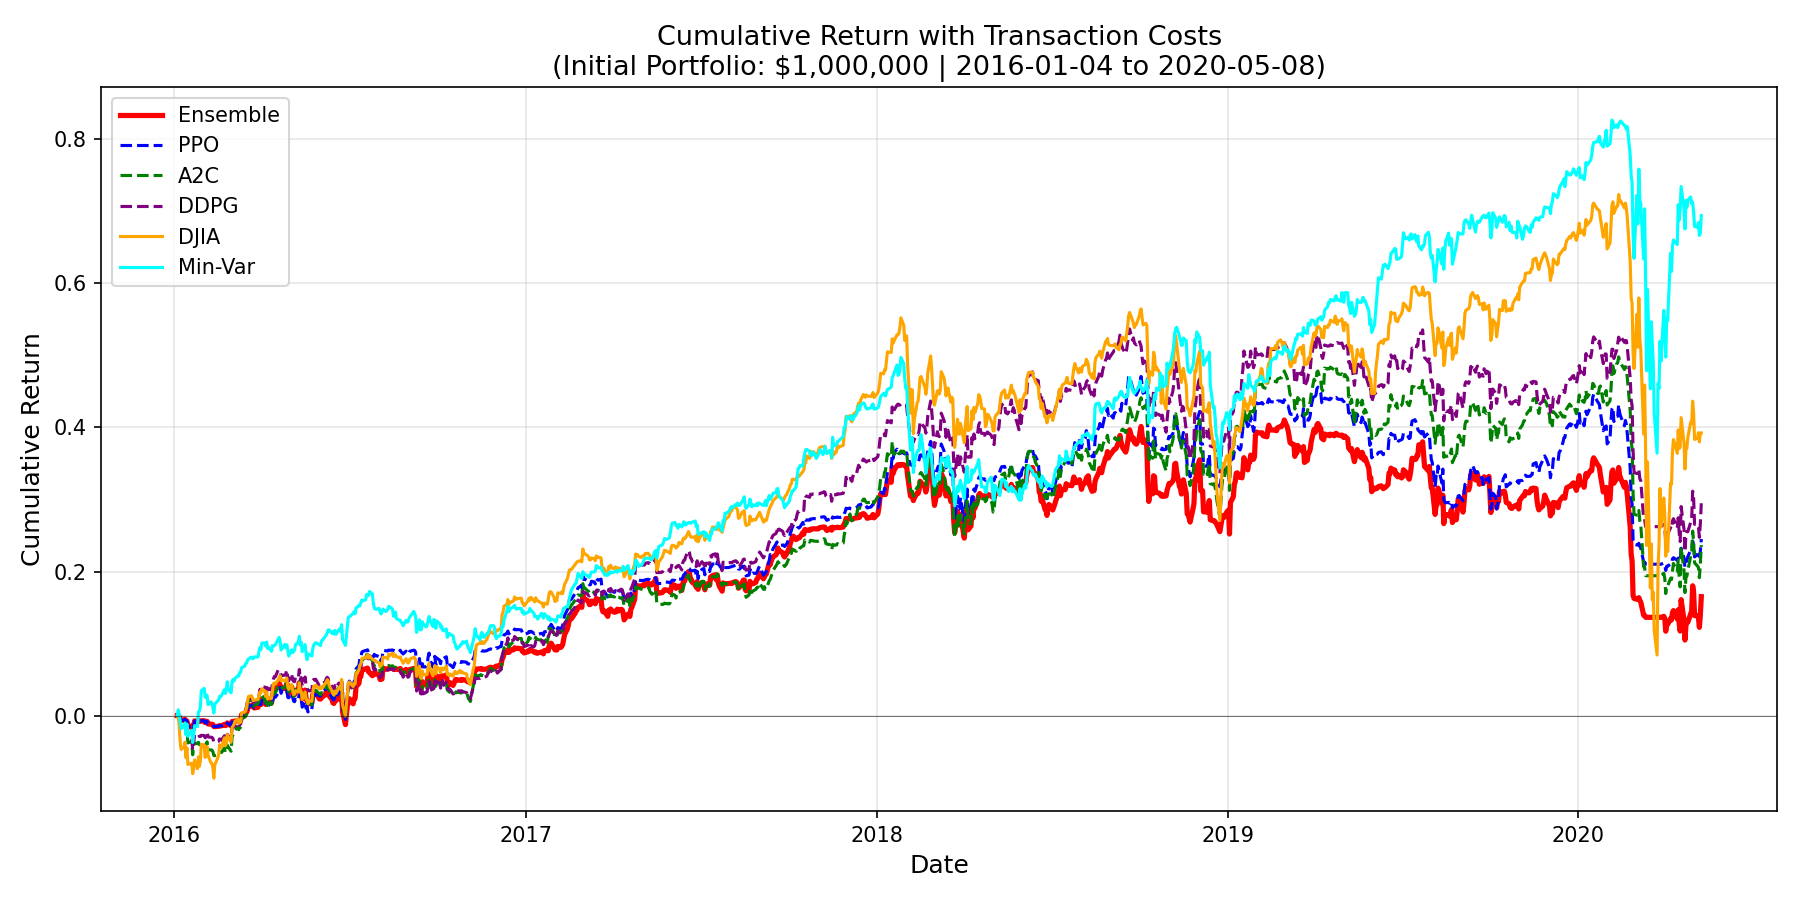
\includegraphics[width=0.82\linewidth]{outputs/cumulative_returns.png}
  \caption{Cumulative return curves with 0.1\% transaction cost.
           Initial portfolio value: \$1,000,000.}
  \label{fig:cumret}
\end{figure}

\begin{table}[H]
\centering
\caption{Performance comparison: replication vs.\ original paper (2016/01/04--2020/05/08).}
\label{tab:perf}
\small
\begin{tabular}{lrrrrrrr}
\toprule
 & \multicolumn{2}{c}{Cum.\ Return} & \multicolumn{2}{c}{Sharpe Ratio} &
   \multicolumn{2}{c}{Max Drawdown} \\
\cmidrule(lr){2-3}\cmidrule(lr){4-5}\cmidrule(lr){6-7}
Strategy & Ours & Paper & Ours & Paper & Ours & Paper \\
\midrule
Ensemble  & 16.5\% & 70.4\% & 0.38 & 1.30 & $-$21.7\% & $-$9.7\%  \\
PPO       & 24.5\% & 83.0\% & 0.55 & 1.10 & $-$18.3\% & $-$23.7\% \\
A2C       & 23.7\% & 60.0\% & 0.47 & 1.12 & $-$21.9\% & $-$10.2\% \\
DDPG      & 29.5\% & 54.8\% & 0.57 & 0.87 & $-$20.1\% & $-$14.8\% \\
DJIA      & 39.2\% & 38.6\% & 0.51 & 0.47 & $-$37.1\% & $-$37.1\% \\
Min-Var   & 69.4\% & 31.7\% & 0.90 & 0.45 & $-$25.3\% & $-$34.3\% \\
\bottomrule
\end{tabular}
\end{table}

We additionally implemented the paper's quarterly rolling-retrain strategy
using 100,000/50,000 timesteps per quarter (PPO/A2C and DDPG respectively).
Full results are reported in Appendix~C (Table~\ref{tab:retrain},
Figure~\ref{fig:retrain}). The rolling ensemble achieved Sharpe~0.24,
\emph{lower} than every fixed-model agent, a finding discussed in Section~4.

%──────────────────────────────────────────────────────────────────
\section{Critical Comparison and Discussion}
%──────────────────────────────────────────────────────────────────

\textbf{Validation.}
The DJIA benchmark replicates almost exactly (Sharpe 0.51 vs.\ 0.47,
max drawdown $-37.1\%$ vs.\ $-37.1\%$), confirming that environment,
data pipeline, and metrics are correctly implemented.
Performance gaps in the RL strategies therefore reflect genuine
methodological differences rather than coding errors.

\textbf{Distributional shift.}
Our RL agents achieve Sharpe ratios of 0.47--0.57 vs.\ 0.87--1.12 in the paper.
The gap stems from the \emph{absence of quarterly retraining}: policies learned
on the high-volatility 2009--2015 recovery period do not generalise to the
low-volatility 2016--2019 bull market, a textbook case of distributional shift.
The paper's rolling retraining is not a computational convenience but a
methodological necessity that the original text does not sufficiently emphasise.

\textbf{Ensemble design dependency.}
Our ensemble ranks last (Sharpe 0.38), inverting the paper's central finding.
Without retraining, the quarterly selection rule merely picks among three
\emph{frozen} policies; the previous-quarter Sharpe becomes a noisy signal
rather than a measure of adaptability.
This reveals that the paper's ensemble outperformance is \emph{inseparable}
from the retraining procedure; the selection logic alone adds no value.

\textbf{Questionable assumptions.}
The assumed 0.1\% transaction cost underestimates realistic execution costs
(bid-ask spreads, market impact) for a \$1M portfolio trading 30 stocks
simultaneously, disproportionately disadvantaging the RL agents which trade
more actively. The universe is also confined to 2016 DJIA constituents,
introducing \emph{survivorship bias}; performance on a broader universe would
likely be lower. The turbulence threshold (140) is not formally calibrated,
and alternative values could materially change the 2020 crash results.

\textbf{Rolling retraining requires adequate compute.}
Our lightweight rolling-retrain experiment (100k/50k steps per quarter)
produced an ensemble Sharpe of 0.24, lower than the fixed-model ensemble
(0.38) and all individual agents.
Each quarterly retrain converges only partially on 100k steps, so the
selection rule consistently promotes an undertrained policy over a mature
one. This confirms that the paper's ensemble advantage is inseparable from
a sufficient per-quarter training budget ($\sim$500k steps); the selection
logic alone, applied to inadequately trained models, adds no value and can
actively reduce performance.

\textbf{Min-variance and regime dependence.}
Min-variance achieves Sharpe 0.90 (vs.\ 0.45 in the paper), outperforming
all RL strategies in our replication.
Conservative weights estimated on turbulent 2008--2015 data happen to be
well-suited to the calm 2016--2019 bull market.
This challenges the paper's framing of min-variance as a weak baseline:
the RL advantage is \emph{regime-dependent}, and the paper's results may
partly reflect the specific 2016--2020 window rather than robust superiority
over classical portfolio optimisation.

\newpage
%──────────────────────────────────────────────────────────────────
\section*{References}
%──────────────────────────────────────────────────────────────────
\begin{itemize}
  \item Yang, H., Liu, X.-Y., Zhong, S., \& Walid, A. (2020). Deep reinforcement
        learning for automated stock trading: An ensemble strategy. In
        \textit{Proceedings of the First ACM International Conference on AI in Finance}
        (ICAIF~'20). Association for Computing Machinery.
        \url{https://doi.org/10.1145/3383455.3422540}
  \item Schulman, J., Wolski, F., Dhariwal, P., Radford, A., \& Klimov, O. (2017).
        \textit{Proximal policy optimization algorithms}. arXiv.
        \url{https://arxiv.org/abs/1707.06347}
  \item Mnih, V., Badia, A.~P., Mirza, M., Graves, A., Lillicrap, T., Harley, T.,
        Silver, D., \& Kavukcuoglu, K. (2016). Asynchronous methods for deep
        reinforcement learning. In \textit{Proceedings of the 33rd International
        Conference on Machine Learning} (Vol.~48, pp.~1928--1937). PMLR.
  \item Lillicrap, T.~P., Hunt, J.~J., Pritzel, A., Heess, N., Erez, T., Tassa, Y.,
        Silver, D., \& Wierstra, D. (2016). Continuous control with deep reinforcement
        learning. In \textit{4th International Conference on Learning Representations}.
        \url{https://arxiv.org/abs/1509.02971}
  \item Kritzman, M., \& Li, Y. (2010). Skulls, financial turbulence, and risk
        management. \textit{Financial Analysts Journal}, \textit{66}(5), 30--41.
        \url{https://doi.org/10.2469/faj.v66.n5.3}
\end{itemize}

%──────────────────────────────────────────────────────────────────
\appendix
\section*{Appendix A\quad Quarterly Model Selection}
%──────────────────────────────────────────────────────────────────

\begin{figure}[H]
  \centering
  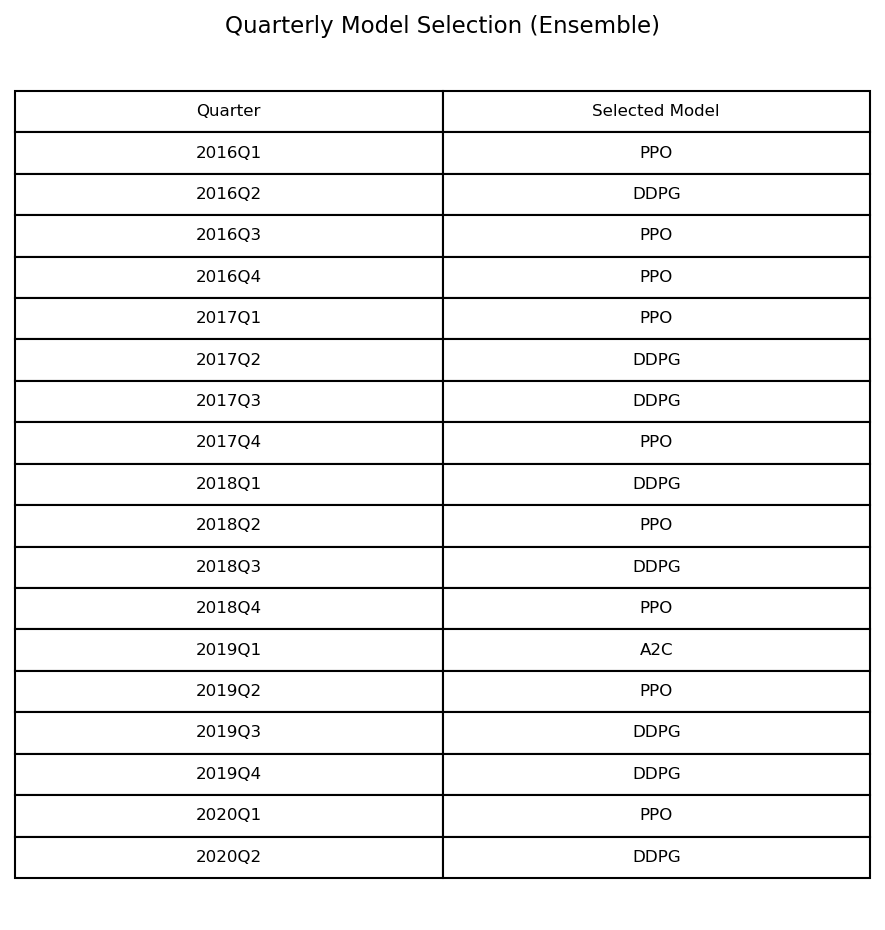
\includegraphics[width=0.45\linewidth]{outputs/model_selection.png}
  \caption{Agent selected each quarter by the ensemble strategy.}
  \label{fig:selection}
\end{figure}

\section*{Appendix B\quad Key Implementation Details}

The full source code is available in \texttt{trading\_replication.py}.
Below is the ensemble quarterly selection logic:

\begin{lstlisting}[caption={Quarterly ensemble: select agent with highest previous-quarter Sharpe.}]
for qi, q in enumerate(unique_quarters):
    if qi > 0:
        prev_returns = agent_daily_returns[prev_quarter]
        best_model = max(agents,
                         key=lambda n: sharpe(prev_returns[n]))
    # Apply selected model's daily returns to ensemble portfolio
    for i in quarter_indices:
        portfolio[i] = portfolio[i-1] * (1 + agent_returns[best_model][i])
\end{lstlisting}

\section*{Appendix C\quad Rolling Retrain Results}

Table~\ref{tab:retrain} and Figure~\ref{fig:retrain} compare the quarterly
rolling-retrain ensemble against the fixed-model strategies over 2016--2020.
PPO, A2C, and DDPG columns show the same pre-trained fixed models for
reference; only the ensemble policy changes each quarter.

\begin{table}[H]
\centering
\caption{Rolling quarterly retrain vs.\ fixed-model strategies (2016--2020).
         100k steps for PPO/A2C and 50k for DDPG per quarter.}
\label{tab:retrain}
\small
\begin{tabular}{lrrr}
\toprule
Strategy         & Cum.\ Return & Sharpe & Max Drawdown \\
\midrule
Rolling Ensemble & 8.4\%  & 0.24 & $-$18.3\% \\
PPO  (fixed)     & 24.5\% & 0.55 & $-$18.3\% \\
A2C  (fixed)     & 23.7\% & 0.47 & $-$21.9\% \\
DDPG (fixed)     & 29.5\% & 0.57 & $-$20.1\% \\
DJIA             & 39.2\% & 0.51 & $-$37.1\% \\
Min-Var          & 69.4\% & 0.90 & $-$25.3\% \\
\bottomrule
\end{tabular}
\end{table}

\begin{figure}[H]
  \centering
  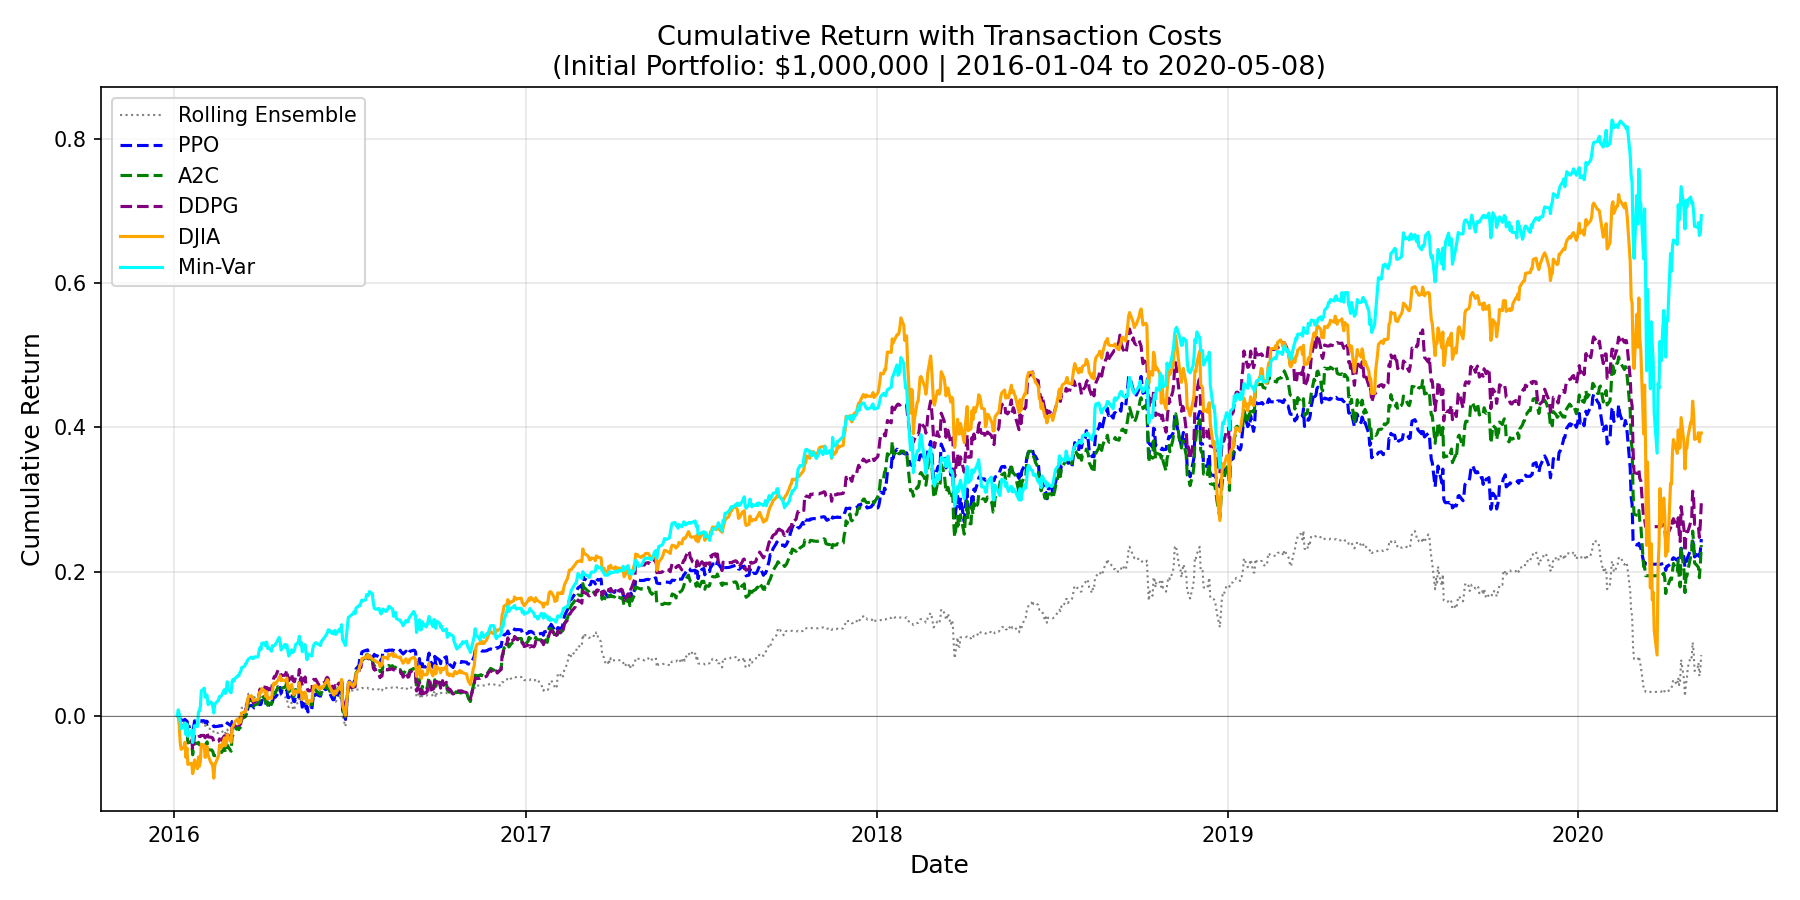
\includegraphics[width=0.82\linewidth]{outputs/cumulative_returns_retrain.png}
  \caption{Cumulative returns with quarterly rolling retraining (100k/50k steps).}
  \label{fig:retrain}
\end{figure}

\end{document}
